\chapter{Mt. Gagazet}
\begin{enumerate}
  \item Walk up, \cs[3:40], walk up, \sd
\end{enumerate}
\begin{battle}{Biran and Yenke}
  \begin{itemize}
    \kimahrif Steal from Biran
    \item Gem Yenke
    \item Gem Biran
  \end{itemize}
  Pay attention to your drops, they affect \yuna's sphere grid below.
\end{battle}
\begin{enumerate}[resume]
  \item \formation{\tidus}{\kimahri}{\wakka}
  \item Make sure you charge \rikku's \od
\end{enumerate}
\end{multicols}
\begin{spheregrid}
  \begin{multicols}{2}
    \begin{itemize}
      \luluf
      \begin{itemize}
        \item Move up, unlock the Level 2 Key Sphere
        \item Move down, unlock the Level 3 Key Sphere to the left of Bribe
        \item Move to the first Str+4 node
      \end{itemize}
      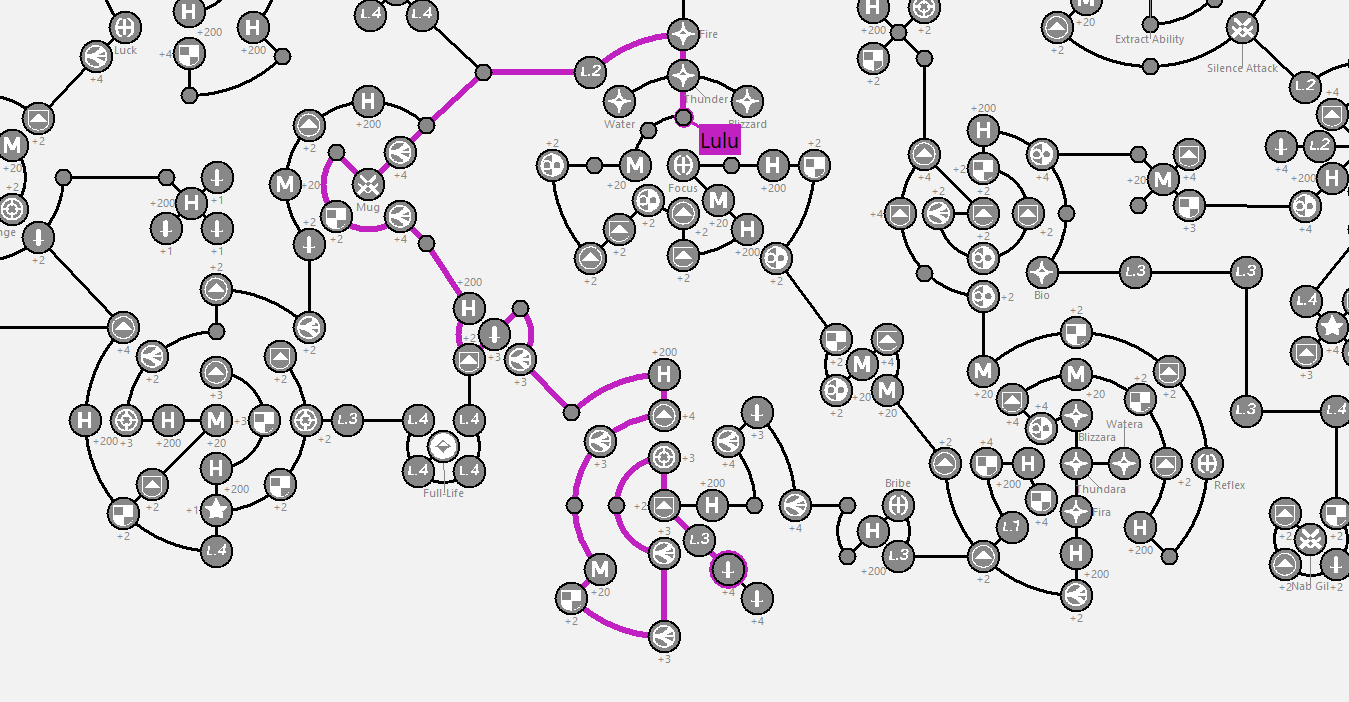
\includegraphics[width=.75\columnwidth]{graphics/lulu_grid}
      \yunaf
      \begin{itemize}
        \item \textit{If you got \textbf{4 Return Spheres}:}
              \begin{itemize}
                \item Return to the last Str+2 node in \wakka's grid ($\downarrow \downarrow \rightarrow \rightarrow \downarrow \downarrow$)
                \item Move left
                \item Mag+3, Level 1 Key Sphere
                \item Move down
                \item Str+2, Agi+4
              \end{itemize}
              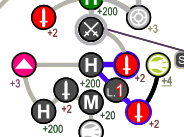
\includegraphics[width=.5\columnwidth]{graphics/4_returns}
              \columnbreak
        \item \textit{If you got \textbf{2 Return Spheres}:}
              \begin{itemize}
                \item Friend Sphere to \lulu
                \item Str+4, Str+4
                      \luluf Go to Str+3
                      \yunaf Friend Sphere to \lulu
                \item Str+3, Agi+4, Agi+4
              \end{itemize}
              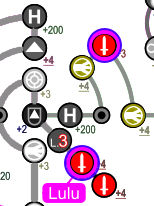
\includegraphics[width=.4\columnwidth]{graphics/2_and_2}
        \item \textit{If you got \textbf{0 Return Spheres}:}
              \begin{itemize}
                \tidusf Move to Str+4 by Armor Break
                \yunaf Friend Sphere to \tidus
                \item Str+4
                      \tidusf Move to Armor Break
                \item Armor Break
                \item Move to Str+4 Below
                      \yunaf Friend Sphere to \tidus
                \item Str+4, Def+3
                \item Do the above \textbf{2 Return Sphere} Menu
              \end{itemize}
              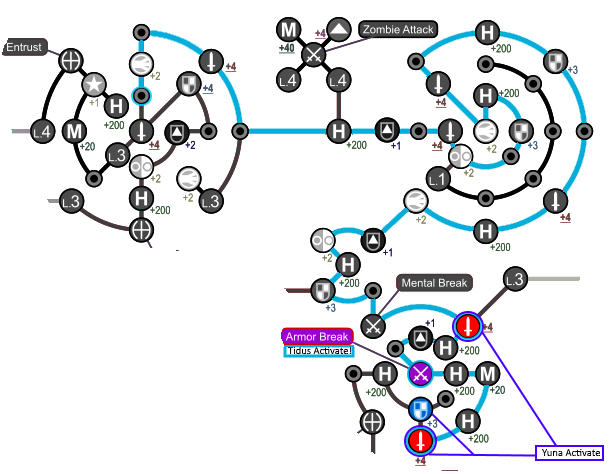
\includegraphics[width=.9\columnwidth]{graphics/0_returns}
      \end{itemize}
      \tidusf: Move to Armor Break and get it if not done already
    \end{itemize}
  \end{multicols}
\end{spheregrid}
\begin{multicols}{2}
\begin{equip}
  \begin{itemize}
    \item Auron: Shimmering Blade
  \end{itemize}
\end{equip}
\begin{enumerate}[resume]
  \item \textit{If you had 2/4 Return Spheres:}
        \begin{itemize}
          \item \formation{\tidus}{\yuna}{\auron}
          \item Customize:
                \begin{itemize}
                  \auronf Shimmering Blade $\rightarrow$ First Strike
                  \yunaf Staff $\rightarrow$ First STrike
                \end{itemize}
        \end{itemize}
  \item \textit{If you had 0 Return Spheres:}
        \begin{itemize}
          \item \formation{\tidus}{\kimahri}{\auron}
        \end{itemize}
  \item Walk up, \sd, \cs[1:20], continue walking up, avoid the gravestones.
  \item Follow the path around, \save, \sd
\end{enumerate}
\vfill
\begin{battle}[70000]{Seymour Flux}
  \begin{itemize}
    \item \textit{If you had 2/4 Return Spheres:}
          \begin{itemize}
            \yunaf Attack
            \tidusf Haste \yuna
            \switch{\auron}{\rikku}
            \rikkuf Silence Grenade or \od\ HP Sphere + Grenade
            \summon{\bahamut}
            \bahamutf Impulse \textit{unless \rikku\ \od\ then } Attack
            \yunaf Attack
            \tidusf Attack. If \yuna\ crit, skip the second Attack to try and get Overkill
          \end{itemize}
    \item \textit{If you had 0 Return Spheres:}
          \begin{itemize}
            \switch{\tidus}{\yuna}
            \summon{\bahamut}
            \bahamutf Attack
          \end{itemize}
  \end{itemize}
\end{battle}
\begin{enumerate}
  \item \textit{If you had 0 Return Spheres:} \formation{\tidus}{\kimahri}{\auron}
  \item Walk to the next screen. \skippablefmv[0:20], \sd, walk up to \tidus\ House, go into the center, \sd. Follow the boy outside, speak to him upstairs, \sd.
  \item Walk up to the next screen, go up the steps. Go down the left path into the water, \sd, swim up. Go up the steps, play the minigame, return to the previous screen.
  \item \tidus\ can attack Splashers for Power Spheres if needed
  \item Return to Save Sphere, go up and left, then go down the right path, swim up into the next screen. Complete the minigame, \rikku\ Green, \tidus\ Blue, \wakka\ Red. Return.
  \item \formation{\tidus}{\yuna}{\auron}
  \item Go up left path, \sd, continue up the path, \save, go onto the next screen.
\end{enumerate}
\begin{battle}[40000]{Sanctuary Keeper}
  \begin{itemize}
    \yunaf Defend
    \tidusf Armor Break
    \item \textit{If doing \bahamut\ endgame:}
          \begin{itemize}
            \auronf Defend
          \end{itemize}
    \item \textit{If doing Quick Hit endgame:}
          \begin{itemize}
            \switch{\auron}{\rikku}
            \rikkuf Defend
          \end{itemize}
          \summon{\bahamut}
          \bahamutf Attack
  \end{itemize}
\end{battle}